\documentclass{irmmwthzconf}

\title{Abstract Title for IRMMW-THz 2019 16pt Times New Roman}
\author{First A.~Author\authormark{1},
  Second B.~Author\authormark{2}, Jr.,
  and Third C.~Author 11pt\authormark{3}}
\affil[1]{California Institute of Technology, Pasadena, CA, 91125 USA 10pt}
\affil[2]{Northwestern University, Evanston, IL, 60208 USA}
\affil[3]{Huntington Medical Research Institutes, Pasadena, CA, 91105 USA}

% only required for the blue URLs in the sample document
% see https://tex.stackexchange.com/questions/23208/i-cannot-get-a-
% properly-underlined-hyperlink-in-blue
\usepackage[super]{nth}
\usepackage{xcolor}
\usepackage[normalem]{ulem}
\let\url\relax
\makeatletter
\DeclareUrlCommand\url@@{%
  \def\UrlFont{\small\color{blue}}%
  \def\UrlLeft{\uline\bgroup}%
  \def\UrlRight{\egroup}}
\def\url@#1{\hyper@linkurl{\url@@{#1}}{#1}}
\DeclareRobustCommand*\url{\hyper@normalise\url@}
\makeatother
% remove if unnecessary

\begin{document}

\maketitle

\begin{abstract}
A short summary (typically 100 words) of the work can go here. Use 9pt bold Times New Roman. A short summary of the work can go here. A short summary of the work can go here. A short summary of the work can go here. A short summary of the work can go here. A short summary of the work can go here.
\end{abstract}

\section{Introduction 10pt small caps}

\IEEEPARstart{T}{his} template should be used for abstract submissions to the \nth{44} \textit{International Conference on Infrared, Millimeter, and Terahertz Waves (IRMMW-THz 2019)} to be held from September 1-\nth{6}, 2019, at Maison de la Chimie, Paris, France. Please refer to the conference website for details, including registration and paper submission information: \url{http://www.irmmw-thz2019.org/}

The Abstract submission document is a template derived from a standard IEEE style template for paper transactions (\url{http://www.ieee.org/web/publications/authors/transjnl/index.html}).

The template is for Microsoft \textit{Word} versions 6.0 or later. Note the page size is 8.5x11'' (US Letter). Please use 10pt Times New Roman throughout the main body text. Leave no blank lines between paragraphs, but indent 2 columns (0.14”). Use single line spacing under paragraph Indents and Spacing. For the initial header use 12pt above, and 4pt below as shown. For future headers use 6pt above and 4pt below as indicated in section II.

\textbf{The length limit for ABSTRACT submissions is one page including text, figures and references.}  Full papers (to be submitted later in a separate upload process) are limited to two pages for regular submissions, three pages for invited Keynote talks, and four pages for invited Plenary talks. These full papers will be included in the conference proceedings, archived on IEEEXplore, and will be distributed to all conference participants.

Abstracts must be submitted in pdf format, and they must be compliant with IEEE PDF standards.  In order to create an IEEE-compliant pdf file, authors should use the IEEE PDF eXpress web site to convert files to pdf format.  Instructions on using this service are available at the `Abstract submission' tab on the conference web site: \url{http://www.irmmw-thz2019.org/}

Please, do not number your pages and do not use any HEADERS or FOOTERS. This section is the Introduction.

\section{Results}

This section describes the results. Use 6pt above and 4pt below the header. This section describes the results. This section describes the results. This section describes the results. This section describes the results. This section describes the results. This section describes the results. This section describes the results. This section describes the results. This section describes the results. This section describes the results. This section describes the results. This section describes the results. This section describes the results. This section describes the results. This section describes the results. This section describes the results.

\textit{Figures:} Format and save your graphic images using a suitable graphics processing program that will allow you to save the images as a jpeg file, for example, and then insert the figure in line with the text using the \textit{Insert $\rightarrow$ Picture $\rightarrow$ From-File} menu. Label Figures with a text box as shown. The column width is 3.5'' with 0.2'' between columns. Be sure your figure and text box fit within this margin.

\begin{figure}[h!]
  \centering
  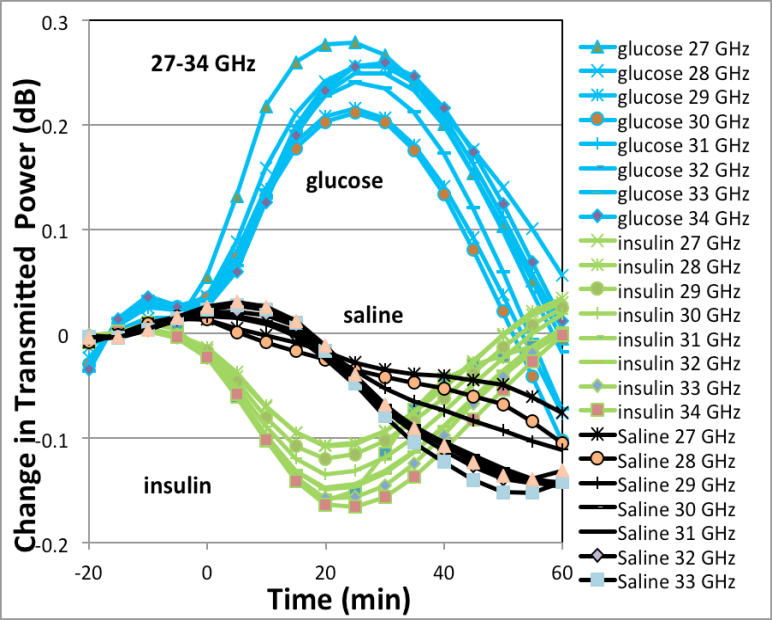
\includegraphics[width=\columnwidth]{transmission.png}
  \caption{Change in millimeter-wave transmission through the animal ear as a
    function of time for various frequencies between 27-34 GHz. At time t=0
    injections were given of: 2g/kg Glucose (blue), 1 ml Saline (black) and 2
    Units/kg Insulin (green). Typical absorption time is 20 minutes. Note that
    the levels track the expected shift in absorption due to change in the
    imaginary part of the index of refraction, consistent with prior data
    from published millimeter wave measurements on blood glucose (see text).}
  \label{fig:transmission}
\end{figure}

\section{Summary}

Add a summary here if you have room. Add a summary here if you have room. Add a summary here if you have room. Add a summary here if you have room. Add a summary here if you have room.

\section{Final Abstract}

Extend the Final Abstract Submissions to two pages. Extend the Final Abstract Submissions to two pages. Extend the Final Abstract Submissions to two pages.

Extend the Final Abstract Submissions to two pages. Extend the Final Abstract Submissions to two pages. Extend the Final Abstract Submissions to two pages. Extend the Final Abstract Submissions to two pages.

Extend the Final Abstract Submissions to two pages. Extend the Final Abstract Submissions to two pages. Extend the Final Abstract Submissions to two pages. Extend the Final Abstract Submissions to two pages.

Extend the Final Abstract Submissions to two pages. Extend the Final Abstract Submissions to two pages. Extend the Final Abstract Submissions to two pages. Extend the Final Abstract Submissions to two pages.

Extend the Final Abstract Submissions to two pages. Extend the Final Abstract Submissions to two pages. Extend the Final Abstract Submissions to two pages. Extend the Final Abstract Submissions to two pages.~\cite{sample, so2012recent, topsakal2011}

\bibliographystyle{IEEEtran}
\bibliography{literature.bib}

\end{document}
